\documentclass[12pt]{article}

%\usepackage[english]{babel}
\usepackage[utf8]{inputenc}
%\usepackage{amsmath}
\usepackage{graphicx}

\title{Supplementary: Effect of needle shape on the trap performance}

%\author{You}

%\date{\today}

\begin{document}
\maketitle

\section{Introduction}

In section IV D of the text we concluded that the needle tip radius of curvature and the taper profile of the needles affect the performance of the trap insignificantly and that the only design parameter of interest ( for the z-potential) is the needle tip-to-tip distance. 
In this short supplementary we provide justification for this claim. 
We study the potential created by a pair of needles near the center of the trap by solving the Laplace equation numerically. 
The boundary conditions are set by applying 1 volt on the needle surfaces. 
Fig 1 a), b) show the potential for a pair of needle in the XZ plane and along the z-axis respectively. 

To compare different potentials, we fit the potential along the z-axis to a harmonic potential of the form $ \frac{1}{2} m \omega_Z^2 z^2$. Where m is the mass of a single $^{171}$Yb$^+$ ion. The trap frequency $\omega_z$ characterizes the strength of the potential.

We consider the effect of the following parameters in the trap potentials:

\begin{itemize}
    \item Needle tip radius of curvature
    \item Asymmetry in the tip radii of curvature of two needles in a trap
    \item Specific needle taper profile
\end{itemize}

\begin{figure}
    \centering
    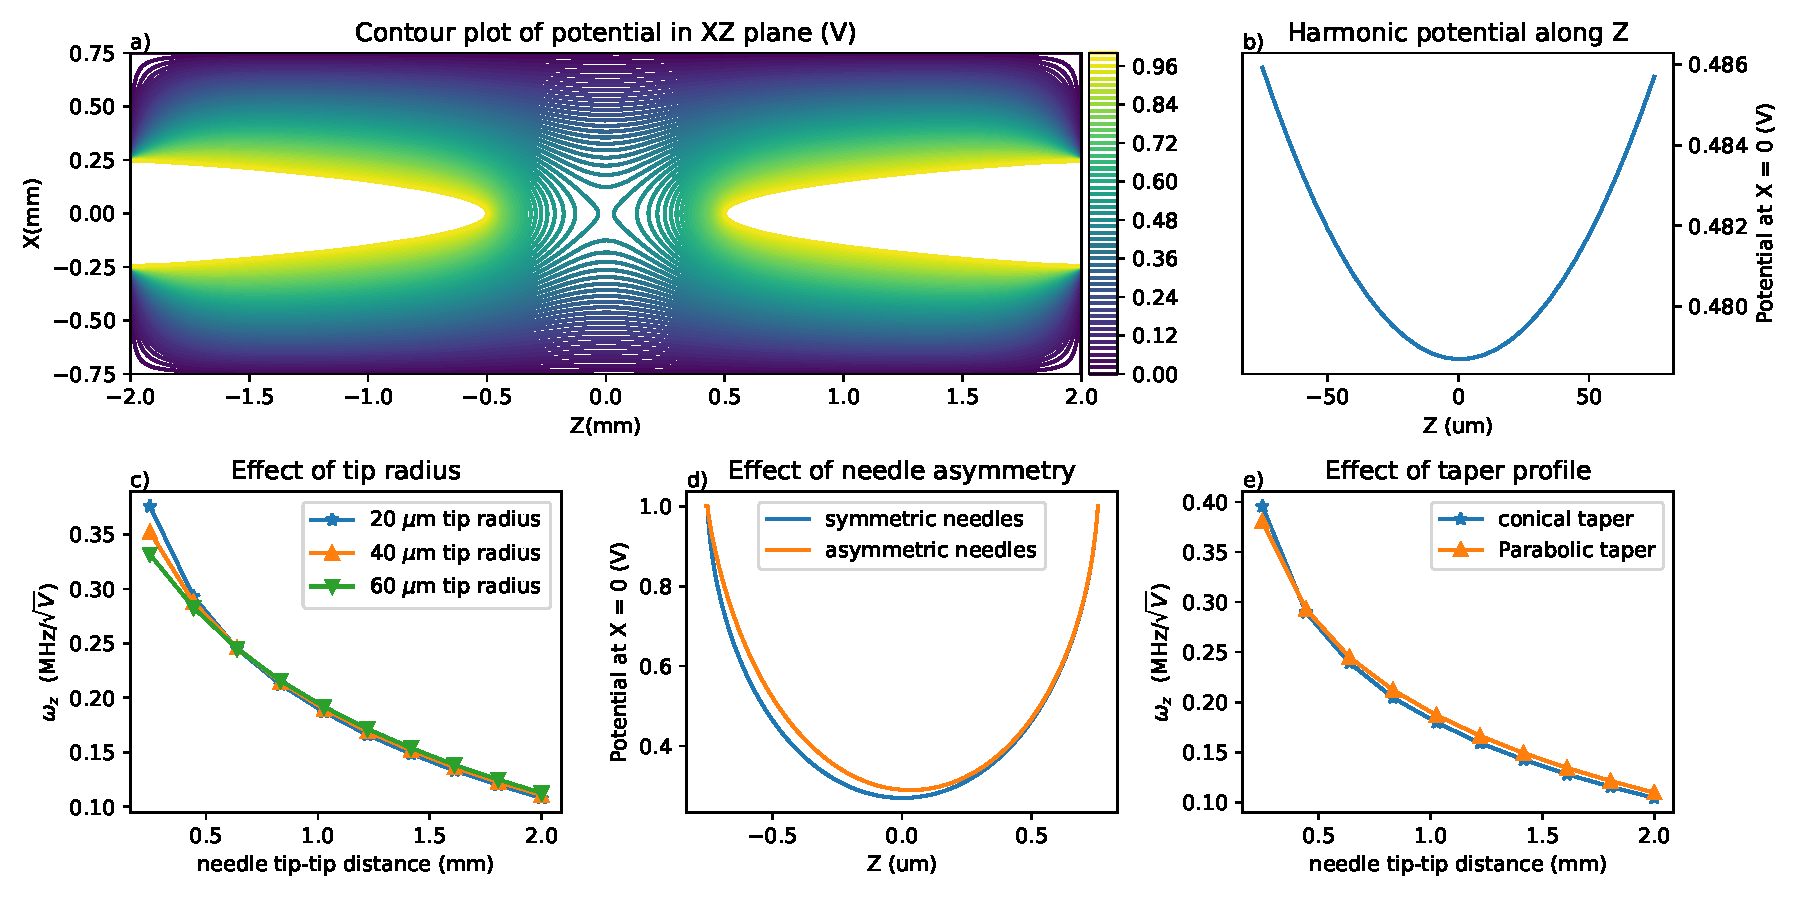
\includegraphics[width = \linewidth]{needle_shape_study.pdf}
    \caption{Effect of needle shape/position on potential along Z-axis}
    a) Contour plot of potential created by a pair of needles in the XZ plane. b) The harmonic approximation holds close to the trapping center c) Tip radius of curvature does not significantly affect the potential for typical tip-tip distances d) Needle asymmetry only shifts the trapping center. The symmetric pair corresponds to two needles with tip radius of curvature of 20 microns and rod end diameter of 250 microns. The asymmetric pair consists one needle with tip of curvature of 60 microns and a rod end diameter of 750 microns. e) The exact shape of taper does not affect the trapping potential appreciably.  
    \label{fig:my_label}
\end{figure}

\section{Results}
Fig 1c) shows the variation of the trap frequency w.r.t the needle tip-tip distance. 
The effect of the needle tip radius of curvature only becomes important below 500 um. 
Since most traps employ needles that a few mm away, the conclusion that the tip radius of curvature plays a negligible role holds. 
For traps where the ion to needle distance is shorter, the intuitive expectation, sharper needles provide stronger confinement, holds. 
However, even with tip-tip distances that are smaller than 500um, the difference in trapping strengths can be readily corrected by applying higher voltages on the needles. 
The needles produced in this work are especially suited for low tip-tip (therefore ion-tip) distances due to their surface finish. 

Fig 1d) shows the potential created by mismatched needles near the trapping region. 
It is clear from the potential along the z-axis that the mismatched needles only affect the location of the minima of the potential and an inconsequential offset to the potential. 
This shows that the requirements for shape matching of the needles are quite relaxed and it may not be prudent to precisely match the needle shapes in a trap for performing high quality QIP research.

Finally the exact taper profile of a needle also does not affect the potentials significantly. 
This is clear from the fig 1e).
The tip-tip distance affects the potentials much more drastically compared to the specific form of the taper.

\section{Conclusion}
We analyzed the effect of the needle shapes and tip radii of curvature on the potentials created in the trapping region.
It is concluded that for ion traps used for performing QIP experiments, the main design parameter for varying z-axis potential is the tip-tip distance of the needles.
From the main text it is also clear that the axial alignment of the needles is important for minimizing excess micromotion.
The tip radius of curvature, asymmetry in needle shapes and the specific taper profile do not affect the potential appreciably.
It is therefore recommended to tune the design and manufacturing effort towards tip-tip distance and axial alignment of needles. 

\end{document}